% !TeX spellcheck = de_DE
% \documentclass{CPS-Beamer}
\documentclass[aspectratio=169]{CPS-Beamer}
% \documentclass[plain]{CPS-Beamer}

\mode<presentation>

\usepackage[ngerman]{babel}
\usepackage[T1]{fontenc}
\usepackage[utf8]{inputenc}
\usepackage{fancyvrb}
\title{Adding Opcodes to RISCV-Toolchain}
\subtitle{Basic Introduction}

\author[Pieper]{Pascal Pieper \\
{\tiny Pascal.Pieper@dfki.de}}
\institute[DFKI CPS]{DFKI GmbH, Cyber-Physical Systems \\ www.dfki.de/cps}

%\date[ISPN '80]{27th International Symposium on Prime Numbers, --280}

\begin{document}

\maketitle

\section{Overview}

\begin{frame}{Overview}
	\begin{block}{}
		\begin{itemize}
			\item Choose a fitting instruction format (see fig. \ref{formats})
			\item Add custom instruction name and bitformat to \texttt{custom-opcodes} 
			\item Insert generated bitmasks into \texttt{riscv-opc.h} 
			\item Add assembler commands to \texttt{riscv-opc.c} 
		\end{itemize}
	\end{block}
\end{frame}

\begin{frame}{Instruction Types}%[plain]
	\vspace{1em}
	\begin{figure}
		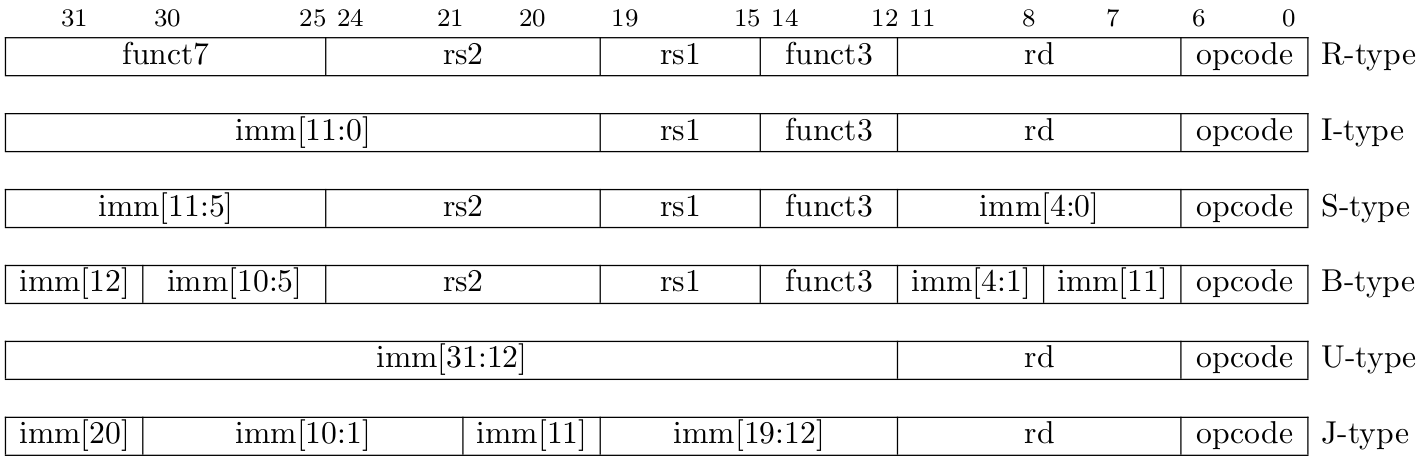
\includegraphics[width=\textwidth]{RiscV_Types.png}
		\caption{\label{formats}RISC-V base instruction formats showing immediate variants}
	\end{figure}
\end{frame}

\section{Custom Opcode}
\begin{frame}[fragile]{Custom Opcode}
	\begin{block}{\texttt{/riscv-opcodes/opcodes-custom}}
		\begin{itemize}
			\item choose applicable opcode (\texttt{6..2}, see fig. \ref{opcodes})
			\item Add custom instruction name and format to \texttt{custom-opcodes}
			\item[$\rightarrow$] Operation code $\neq$ Assembler instruction!
		\end{itemize}
File \textit{custom-opcodes:}
\begin{verbatim}
# Operation   rd source1  source2   func3    code     non-compressed
settaint.i    rd 19..15=0 imm12    14..12=0 6..2=0x0A 1..0=3  #I Type
settaint.r    rd rs1      31..20=0 14..12=1 6..2=0x0A 1..0=3  #R-Type
gettaint      rd rs1      31..20=0 14..12=2 6..2=0x0A 1..0=3  #R-Type
\end{verbatim}
\end{block}
\end{frame}


\begin{frame}{Opcodes}%[plain]
	\vspace{1em}
	\begin{figure}
		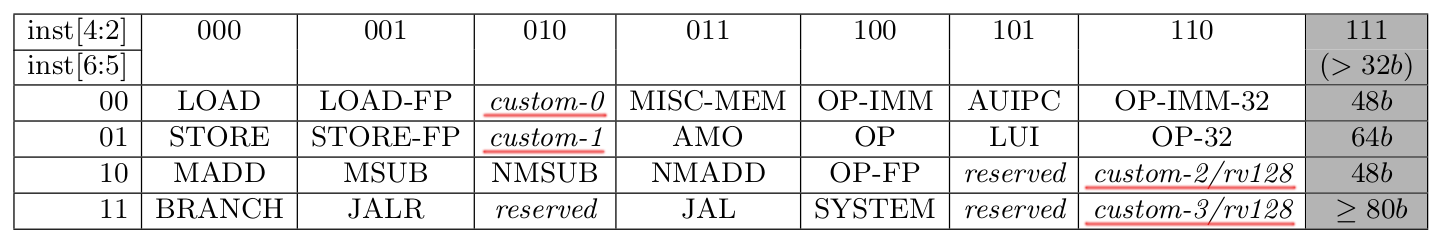
\includegraphics[width=\textwidth]{opcode_map.png}
		\caption{\label{opcodes}RISC-V base opcode map, inst[1:0]=11}
	\end{figure}
\end{frame}

\begin{frame}[fragile]{Custom Opcode}
	\begin{block}{\texttt{/riscv-opcodes/}}
		\begin{itemize}
			\item Run mask generator:
		\end{itemize}
\texttt{\$ cat opcodes-custom | ./parse-opcodes}
\end{block}
\end{frame}


\section{Assembler instruction}
\begin{frame}[fragile]{Assembler instruction}
	\begin{block}{\texttt{/riscv-binutils/include/opcode/riscv-opc.h}}
		\begin{itemize}
			\item Insert generated mask and match bitmasks 
		\end{itemize}
File \textit{riscv-opc.h:}
\begin{verbatim}
...
#define MATCH_SETTAINT_I 0x002b
#define MASK_SETTAINT_I  0xff07f
#define MATCH_SETTAINT_R 0x102b
#define MASK_SETTAINT_R  0xfff0707f
#define MATCH_GETTAINT   0x202b
#define MASK_GETTAINT    0xfff0707f
...
\end{verbatim}
	\end{block}
\end{frame}


\section{Assenbler instructions}
\begin{frame}[fragile]{Assembler instructions}
	\begin{block}{\texttt{/riscv-binutils/opcodes/riscv-opc.c}}
		\begin{itemize}
			\item Add custom assembler instructions
		\end{itemize}
File \textit{riscv-opc.c:}
\begin{Verbatim}[fontsize=\footnotesize]
...
{"add",         0, {"I", 0},   "d,s,j",  MATCH_ADDI, MASK_ADDI, match_opcode, INSN_ALIAS },
//CUSTOM
{"settaint",    0, {"I", 0},   "d,j", MATCH_SETTAINT_I, MASK_SETTAINT_I, match_opcode, 0 },
{"settaint",    0, {"I", 0},   "d,s", MATCH_SETTAINT_R, MASK_SETTAINT_R, match_opcode, 0 },
{"gettaint",    0, {"I", 0},   "d,s", MATCH_GETTAINT  , MASK_GETTAINT  , match_opcode, 0 },

{"la",          0, {"I", 0},   "d,B",  0,    (int) M_LA,  match_never, INSN_MACRO },
...
\end{Verbatim}
	\end{block}
\end{frame}

\section{Build}
\begin{frame}[fragile]{Build}
	\begin{block}{\texttt{/}}
		\begin{itemize}
			\item Configure and Build!
			\item Verify by using the new Instruction in inline assembly
			\begin{itemize}
				\item \texttt{\footnotesize%
asm volatile
(
	"gettaint  \%[x], \%[y]" %
	: [x] "=r" (taintval) %
	: [y] "r" (*word) %
);}
				\item \texttt{riscv/bin/riscv32-unknown-elf-gcc -g test.c -o test}
				\item \texttt{riscv/bin/riscv32-unknown-elf-objdump -dS test} \\~\\
			\end{itemize}
		\end{itemize}
\begin{Verbatim}[fontsize=\small]
	...
	1021c:       0007c783                lbu     a5,0(a5)
	10220:       0007a7ab                gettaint        a5,a5
	10224:       fef407a3                sb      a5,-17(s0)
	...
\end{Verbatim}
	
	\end{block}
\end{frame}

\end{document}
